\chapter{Results}


\section{Workshop Study findings} \label{sec:sections}

\subsection{Learnings}
Beyond the metrics gathered, there were some additional insights gained from the workshop:
\subsubsection{Precisions}
All body measurements used in the workshop were rounded up to 0.5cm ceilings. While this does affect the fit (slightly looser) and efficiency (minimally higher) it does not affect the analysis that much. The reason for this is that this pattern is not machine cut. The target audience is confident beginners and not industrial tailors. Therefore, precise millimetre level cutting was not a fair expectation.

\subsubsection{Ease, Fit and Comfort}
\begin{figure} [H] % opens the figure environment. the '[H]' forces the image to be Here
    \centering % puts the image in the horizontal centre of the page
    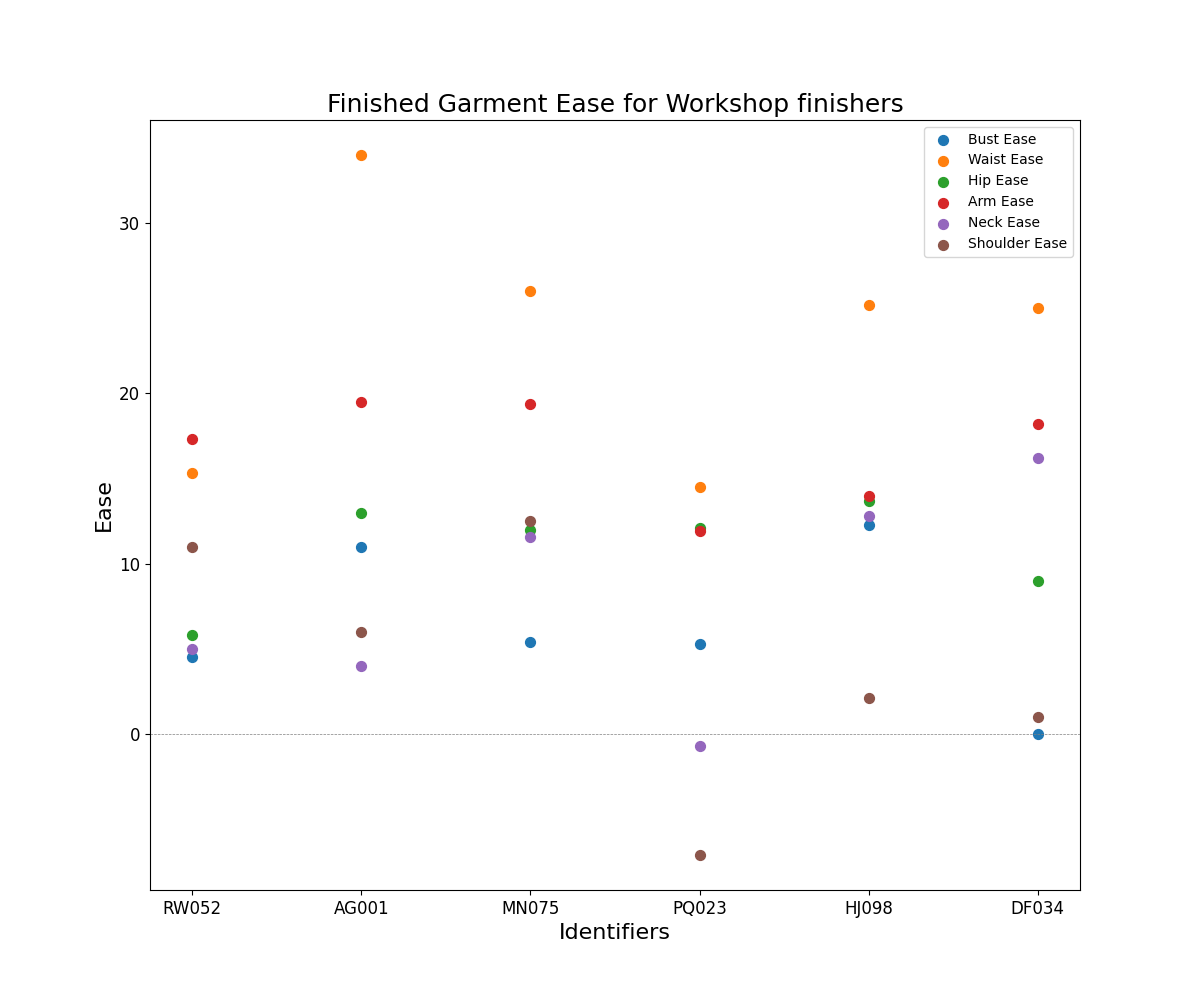
\includegraphics[width = 0.75\textwidth]{Images/FG_Ease_Plot.png} %this tells latex what graphics to include. I put my images in an 'Images' folder to aid file management, hence the Images/ before the file name. the width bit before allows you to alter the width of the image. It is also possible to use scale as well as using equations with the textwidth to make it say half the text width.
    \caption{Finished Garment eases for workshop participants}
    \label{} % this internally labels the figure for future referencing.
\end{figure}

\subsubsection{Fabric Use}
\begin{figure} [H] % opens the figure environment. the '[H]' forces the image to be Here
    \centering % puts the image in the horizontal centre of the page
    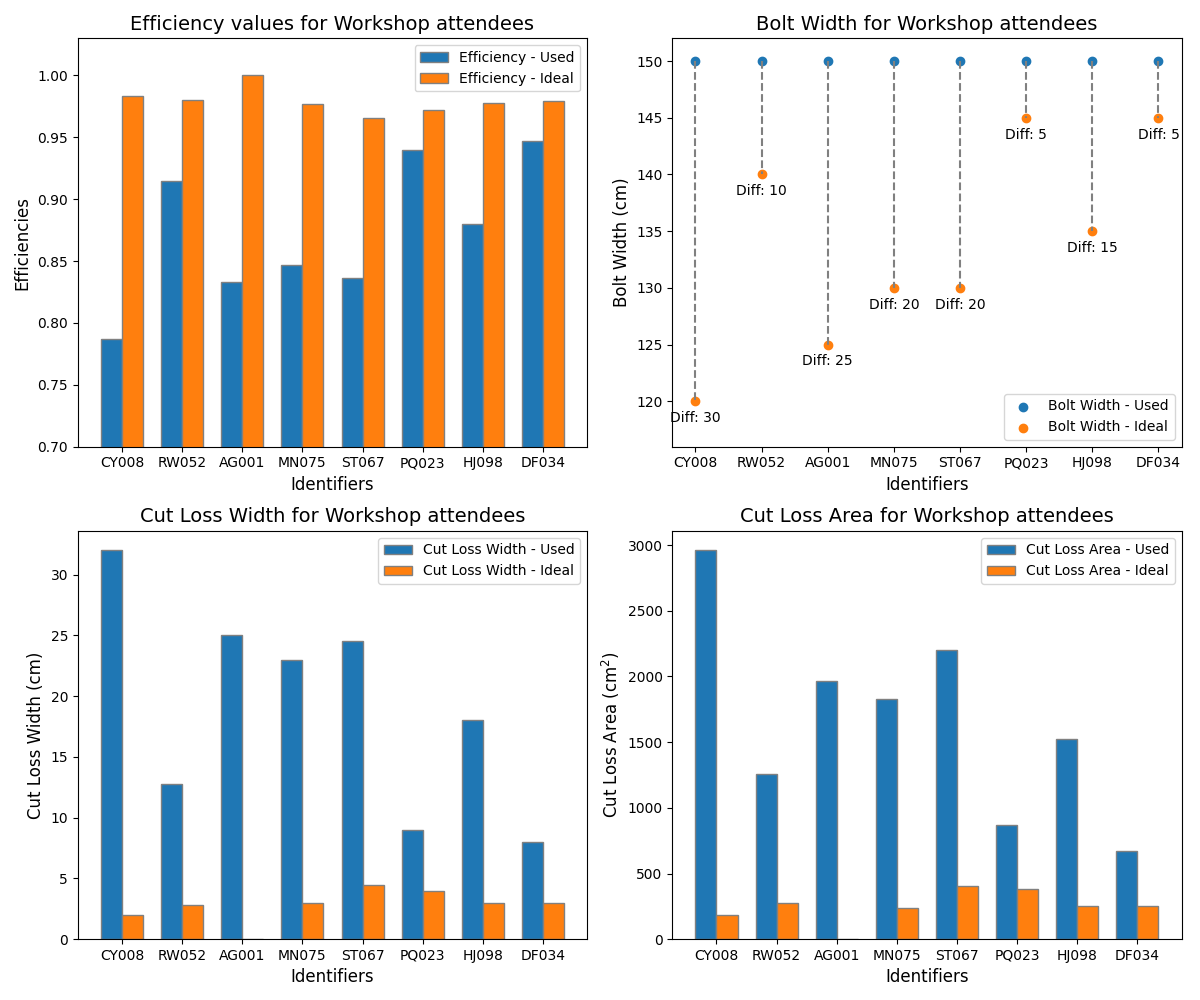
\includegraphics[width = 0.75\textwidth]{Images/Workshop_Plot.png} %this tells latex what graphics to include. I put my images in an 'Images' folder to aid file management, hence the Images/ before the file name. the width bit before allows you to alter the width of the image. It is also possible to use scale as well as using equations with the textwidth to make it say half the text width.
    \caption{Finished Garment eases for workshop participants}
    \label{} % this internally labels the figure for future referencing.
\end{figure}

\subsubsection{Parameterisation Improvements}
Helmersson’s pattern was devised for a rather narrow band of sizes. Some of the elements of the pattern are constant, like the collar, sleevehead curve and the opening for the neck (defined by neck facing). For this project, the pattern had to be generalised for all body shapes and sizes. Scaling factors were applied to these elements which were found to be too aggressive. In retrospect, using neck circumference to influence the neck facing would have been more prudent. This would necessitate changing the seam allowance on the collar piece so that it would align better, especially for smaller necks.
Design ease for the garment width was held at 25 cm. This should have been made more dynamic and responsive to the largest bodice circumference. This is due to the fact that a constant ease feels tighter on a larger body. These changes might positively affect the fit and comfort of the finished garment. Because changing the general ease value also affects finished size of the sleeves, it is difficult to pinpoint the exact adjustments required without further testing. However, the suggestion would be to increase ease for max bodice circumferences above 100 cm and check the theoretical finished garment shoulder width fits the person's measured shoulder with.

\section{100 Body Scans Study findings}
\subsubsection{Distibutions}
\begin{figure} [H] % opens the figure environment. the '[H]' forces the image to be Here
    \centering % puts the image in the horizontal centre of the page
    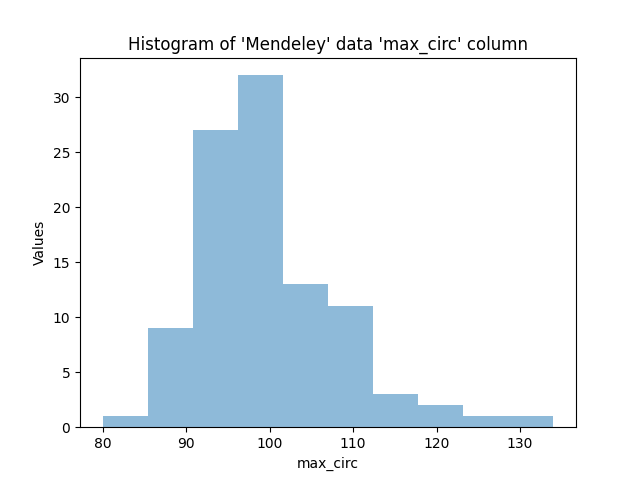
\includegraphics[width = 0.5\textwidth]{Images/Mendeley_max_circ_Hist.png} %this tells latex what graphics to include. I put my images in an 'Images' folder to aid file management, hence the Images/ before the file name. the width bit before allows you to alter the width of the image. It is also possible to use scale as well as using equations with the textwidth to make it say half the text width.
    \caption{Boxplot of max bodice circumference for 100 Scans Study}
    \label{} % this internally labels the figure for future referencing.
\end{figure}
\begin{figure} [H] % opens the figure environment. the '[H]' forces the image to be Here
    \centering % puts the image in the horizontal centre of the page
    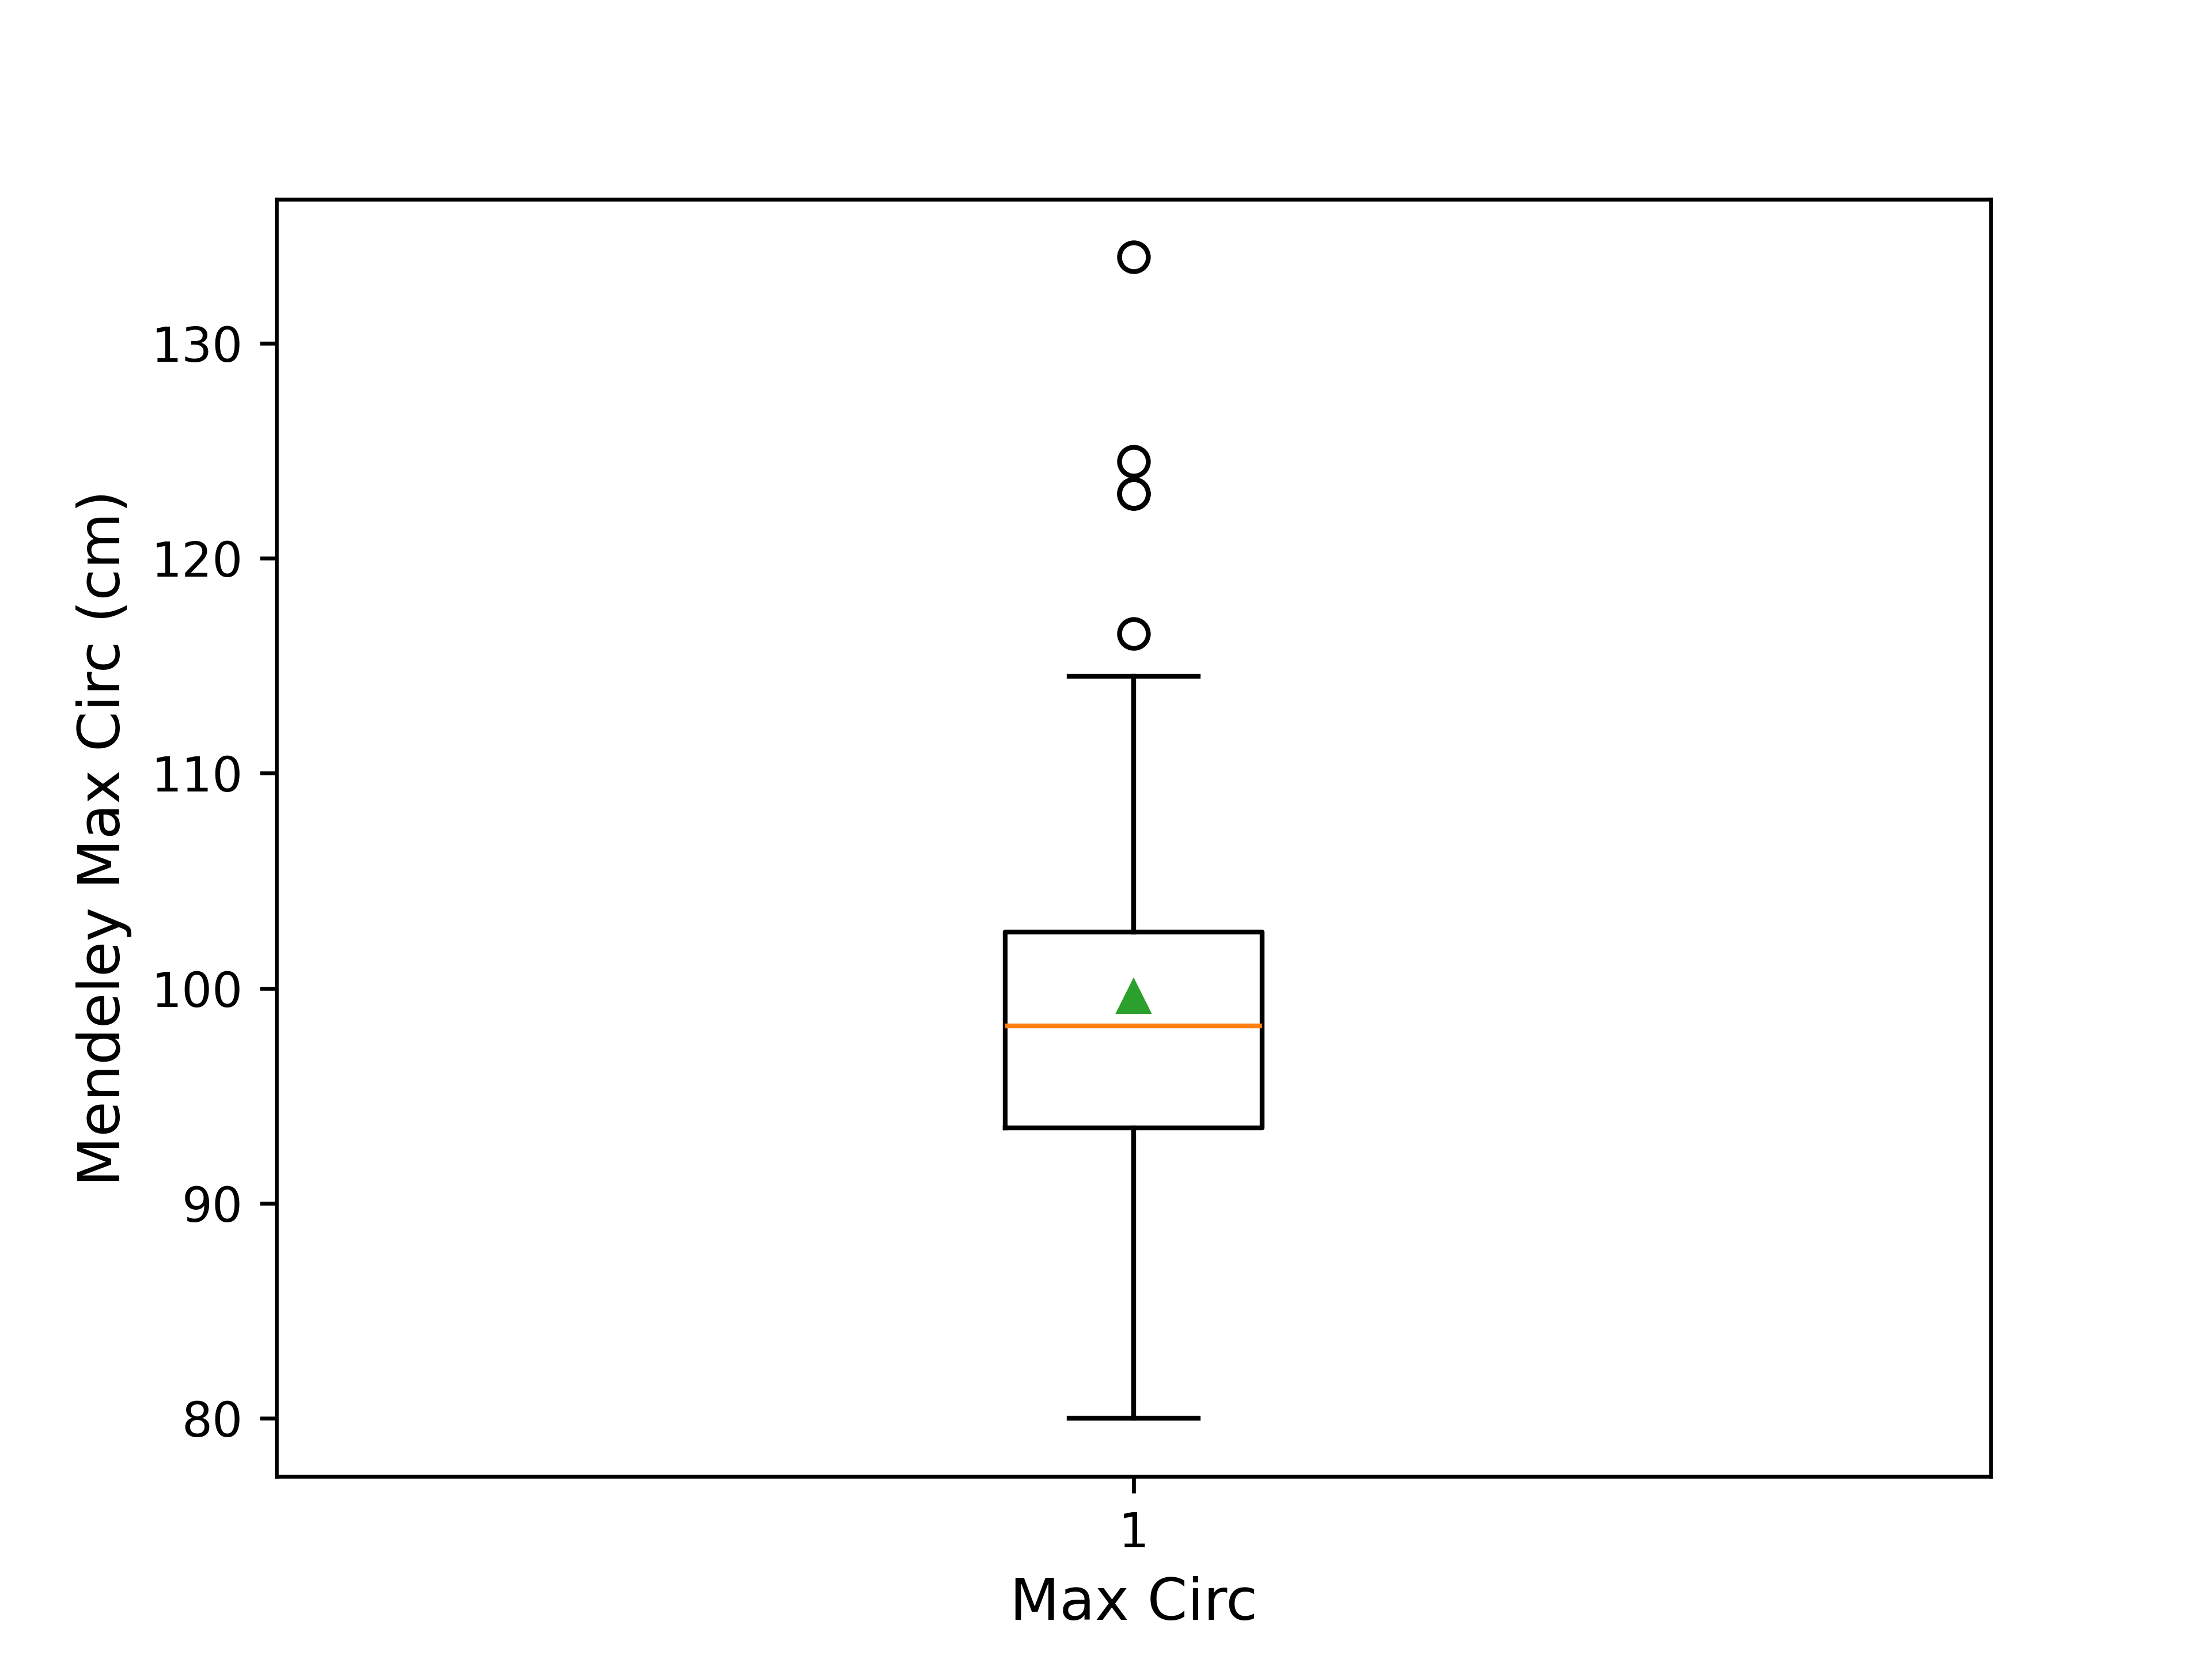
\includegraphics[width = 0.5\textwidth]{Images/Mendeley_max_circ_Boxplot.png} %this tells latex what graphics to include. I put my images in an 'Images' folder to aid file management, hence the Images/ before the file name. the width bit before allows you to alter the width of the image. It is also possible to use scale as well as using equations with the textwidth to make it say half the text width.
    \caption{Boxplot of max bodice circumference for 100 Scans Study}
    \label{} % this internally labels the figure for future referencing.
\end{figure}

\subsubsection{Fabric Use}
\begin{figure} [H] % opens the figure environment. the '[H]' forces the image to be Here
    \centering % puts the image in the horizontal centre of the page
    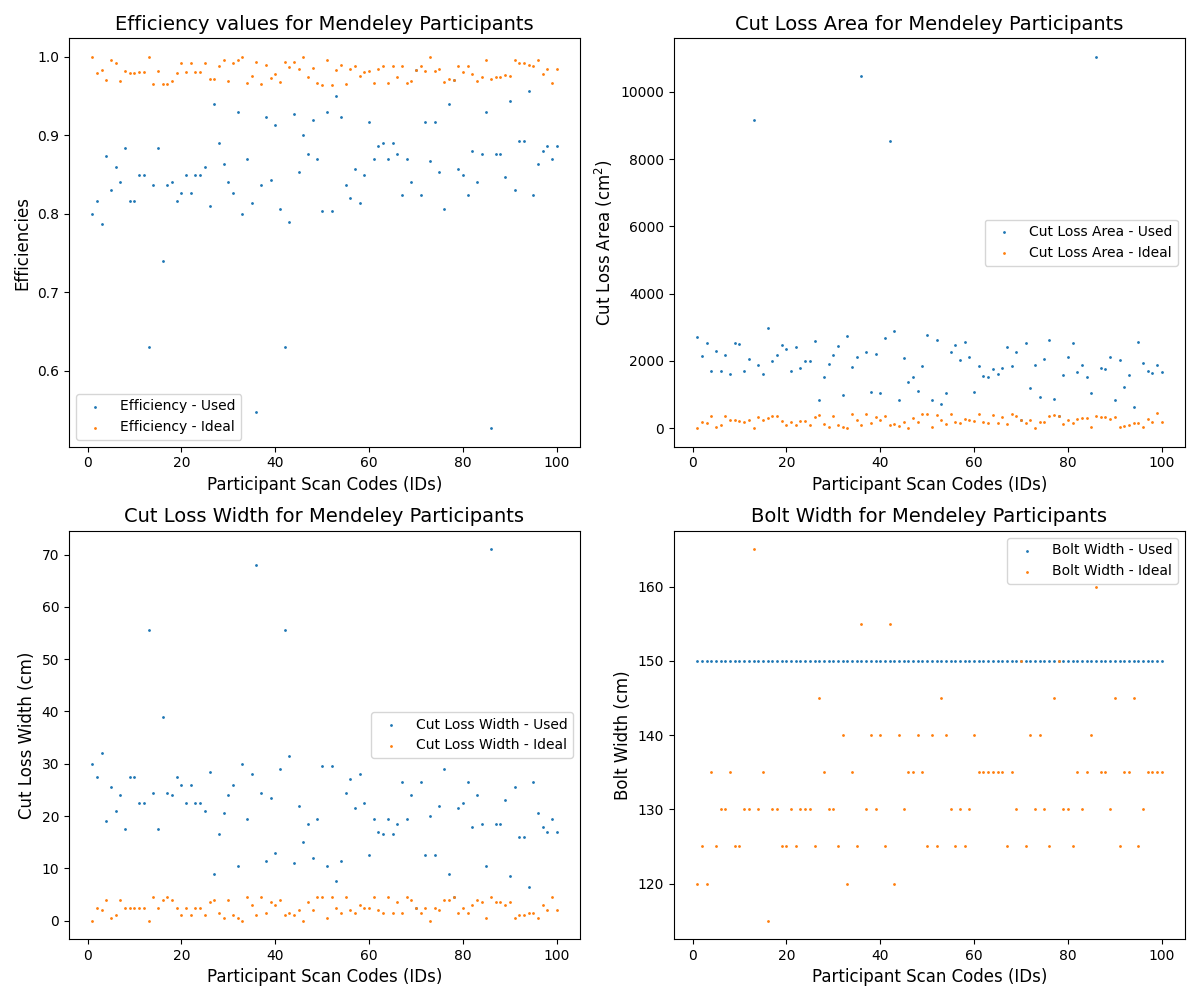
\includegraphics[width = 0.75\textwidth]{Images/Mendeley_Plot.png} %this tells latex what graphics to include. I put my images in an 'Images' folder to aid file management, hence the Images/ before the file name. the width bit before allows you to alter the width of the image. It is also possible to use scale as well as using equations with the textwidth to make it say half the text width.
    \caption{Used and Ideal Efficiency Metrics for 100 Scans Study}
    \label{} % this internally labels the figure for future referencing.
\end{figure}

\begin{figure} [H] % opens the figure environment. the '[H]' forces the image to be Here
    \centering % puts the image in the horizontal centre of the page
    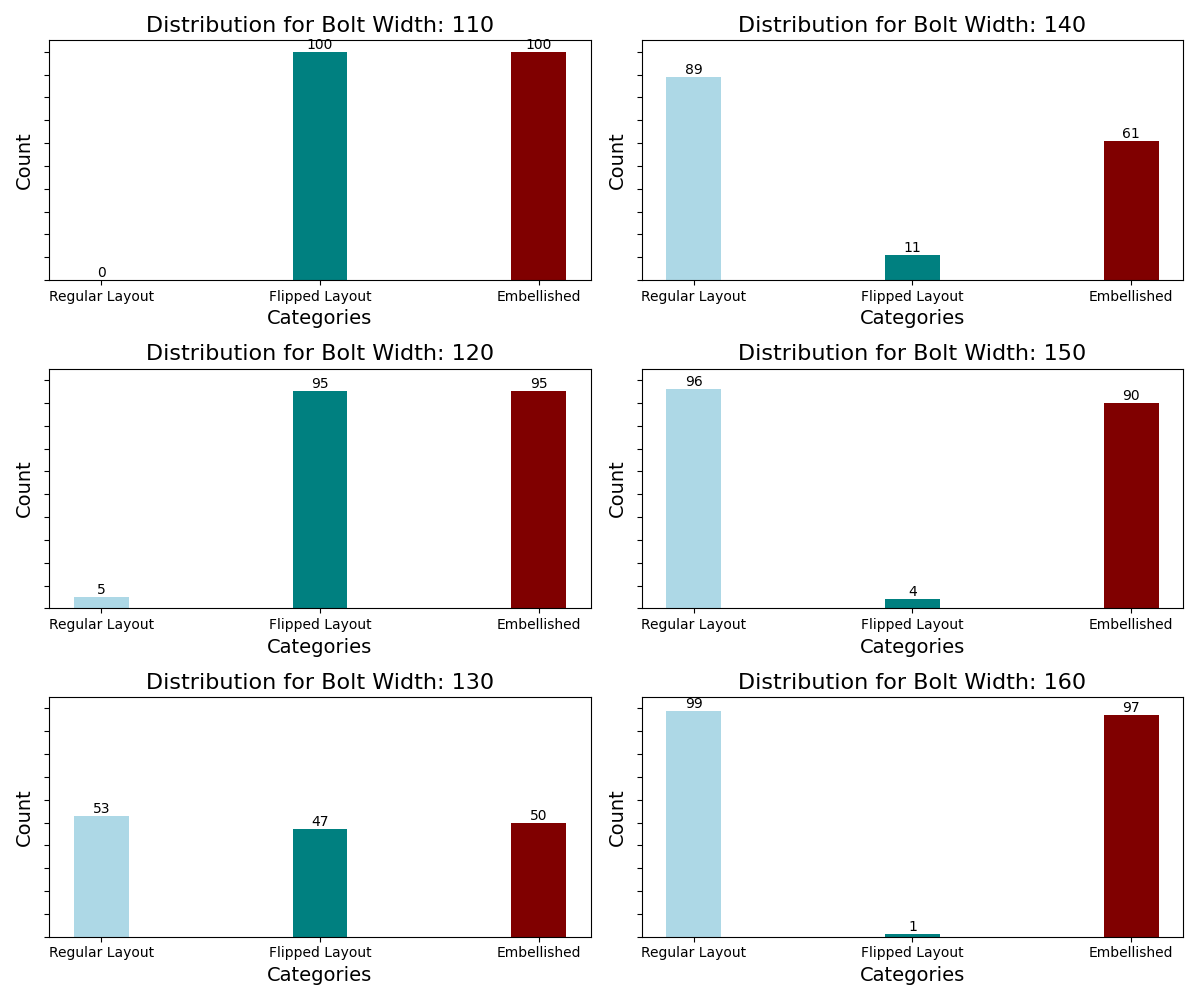
\includegraphics[width = 0.75\textwidth]{Images/Mendeley_Bar.png} %this tells latex what graphics to include. I put my images in an 'Images' folder to aid file management, hence the Images/ before the file name. the width bit before allows you to alter the width of the image. It is also possible to use scale as well as using equations with the textwidth to make it say half the text width.
    \caption{Layout and Embellishment Possibility for 100 Scans Study}
    \label{} % this internally labels the figure for future referencing.
\end{figure}